%!TEX root = thesis.tex
%% %% ***************** Background *****************

%% ************************************************ 2 ************************************************

\section{Background}\label{sec:background}
%\section{Aikaisempi tutkimus}

Machine learning, or ML,
is a subcategory of the AI field and data science.
Typically, ML refers to
a set of technologies used to \enquote{build computers
that improve automatically through experience}.\cite{jordan2015machine}
This is generally considered a machine way
to simulate human learning process.
ML usage has become more common
and is nowadays widely used in many fields,
not just in general information technology and computer science.
This is because data can be gathered from anywhere,
and where there is data to be processed,
ML can be there to process it.
Computer algorithms are able to find 
statistical correlation and patterns
from places overlooked by human mind,
or where amount of data is just too much 
for people to process.
This is why ML has proved its power
in various empirical science fields,
such as biology, cosmology or social science.\cite{jordan2015machine}

In this section, 
key concepts of ML are explained briefly
and several ML features are explored 
that are most relevant to this study.
We also discuss shortly about data sensitivity
and how it had to be addressed during this study.

%% ************************************************************************************************************


\subsection{Machine learning algorithms and training}\label{subsec:bg-machine-learning}

Algorithm means a finite sequence of (typically) mathematical operations
that are used to solve a specific problem,
generally by repetition of some steps
until the problem resolves.\cite{merriam2022algorithm}
Algorithms are the main component inside machine learning~
By iterating through all the data points
algorithm is able to, for example,
find repeating patterns,
mathematical or logical connections,
or unusual anomalies that would be seemingly normal for human eye.

Algorithms operate on set of rules and parameters
In order to utilize an algorithm to solve a problem,
algorithm is first trained by tuning these parameters
to fit the current case.
Usually,
ML algorithms can be trained in three ways:
supervised, unsupervised, and reinforced learning.\cite{jordan2015machine}
Even more training methods exist
that usually combine those mentioned.\cite{ayodele2010types, mahesh2020machine}
For the sake of simplicity,
we focus on those three main methods.

In \textbf{supervised learning},
algorithm is given data with ready answers on
how the data needs to be interpreted.
Algorithm then tries to figure out the rules behind
how given data and the correct answers are related.\cite{ayodele2010types}
In \textbf{unsupervised learning},
on the other hand,
algorithm does not get model data from which to train itself,
but instead it tries to find clusters or groups inside the data
that are linked together more closely than to other data points.\cite{winky}
\textbf{Reinforced learning} refers to a method
where a computer program is given a goal
and provided feedback as a reward.
This reward is what program aims to maximize
by adjusting given parameters.\cite{ayodele2010types}

In ML,
there are multiple algorithms to solve different problems
and no jack-of-all-trades algorithm exists.
Each algorithm is suitable for certain type of problem.
To simplify,
algorithms are usually divided into three or four categories
based on the problem type.\cite{vickery2019mltypes}

\textbf{Regression algorithms} predict values
and are typically used with supervised learning.
Usual example of regression problem
is house price prediction
using typical house features
such as building
year,location, number of rooms \etc.
With these varying features
the algorithm then gives each feature a weight value
which determine the final price of the house.\cite{vickery2019mltypes}

\textbf{Classification algorithms} predict categories
and are also used most commonly with supervised learning.
Depending on the algorithm,
they can predict between two or several categories.
Examples of classification problems
could be spam mail identification with two class classification,
or flower species recognition from images with multiclass classification.\cite{vickery2019mltypes}

\textbf{Clustering algorithms} use unsupervised learning
to find structures inside data.
This is done,
for instance,
by first providing the amount of clusters to search to algorithm,
which then calculates a center point for each cluster
so that they are as far away from each other as possible
while data points surrounding each center are as close to each other as possible.\cite{mahesh2020machine}
This could be used,
for example,
to find meaningful customer segments from transaction data
in order to improve targeted advertising.\cite{chen2017purtreeclust}

\textbf{Dimension reduction algorithms} are a separate type of algorithms used with unsupervised learning,
but they are usually combined with other algorithms
to solve the main problem.
With dimension reduction,
main algorithm calculations are streamlined by first reducing the amount of feature dimensions.\cite{li2017mlalgorithm}

These four ML problem types
and most known algorithms of each type
are shown in the graphic~\ref{fig:ml-algorithm-cheatsheet}.


\begin{figure}[htb]
    \centering
    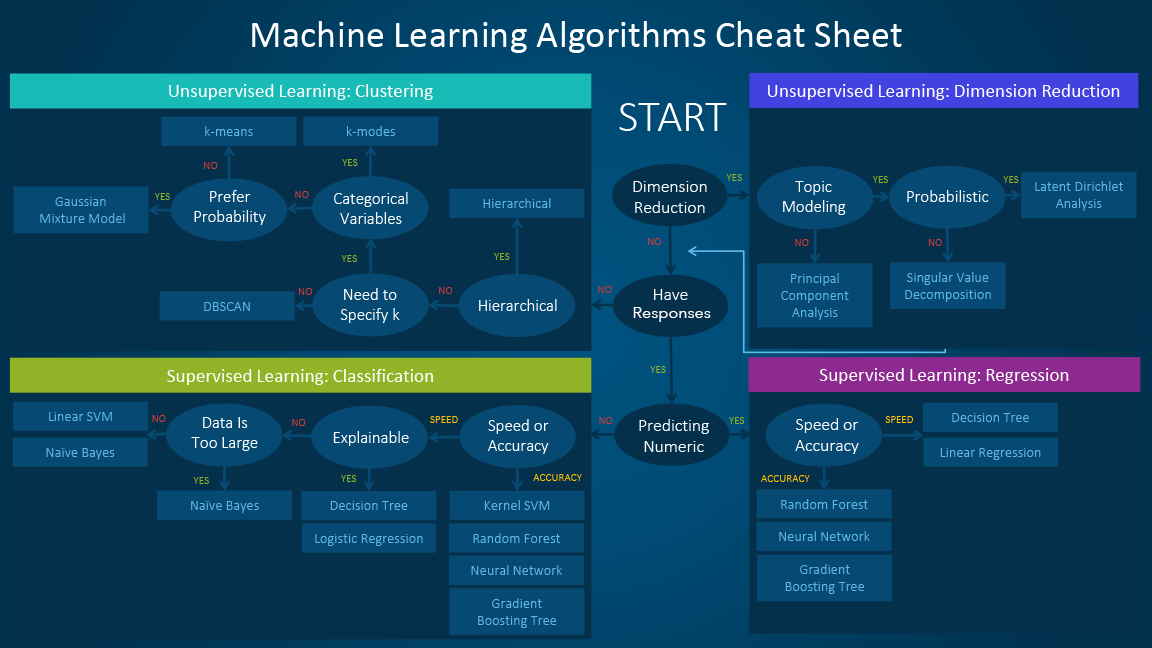
\includegraphics[width=150mm]{./appendices/machine-learning-cheet-sheet-2}
    \caption{Machine learning cheatsheet for algorithm choosing\cite{li2017mlalgorithm}
    \label{fig:ml-algorithm-cheatsheet}}
\end{figure}

This study focuses on anomaly detection,
which, roughly simplified, is a clustering problem
where anomalies are rare incidents outside common clusters.
However,
in this study we utilize PCA-based anomaly detection algorithm,
where PCA refers to Principal Component Analysis,
and which is a dimension reduction algorithm.\cite{li2017mlalgorithm}
More about PCA
is discussed later in this section.
In addition,
we aim to find a connection between anomalies and incident tickets
by their amount in a timeframe,
which makes the topic in the end a regression problem.

Typically,
when training an algorithm,
some predefined portion of the data
is used as training data.
The rest is used to validate the results
so that validation data and training data do not overlap.
Instead, trained algorithm is given data it has not seen before
and the result it produces with it is then validated.\cite{baheti2022datasplit}
For example,
in supervised learning
the key values the algorithm is trained to find out
are hidden from the validation data.
The resulting values produced by the algorithm
are compared to those hidden values
and the difference between the estimate and the real value
can be used to determine how well the current trained algorithm compares to others.
However, in this study,
we are going to break that rule
about non-overlapping training and validation data.
The reason for this is explained further in section~\ref{subsec:pipe-unconventional-training}.

%% ************************************************************************************************************

\subsection{Cloud ML platforms}\label{subsec:bg-cloud-ml-platforms}

Machine learning algorithms are not light to operate.
ML is at its best with big data
where amount of data points
makes it easier for algorithms
to find repeating patterns more reliably.\cite{zhou2017machine}
Data amount, however,
requires huge resources in terms of memory and computing power.
Especially with online applications
where real time analysis of new input data is required
with small latency,
cloud computing can make a big difference
in terms of processing speed.

Online market offers several solutions for ML computing in cloud.
Most notable service providers for
MLaaS (Machine Learning as a Service)
are Google, Amazon, IBM, and Microsoft.
Differences of each service provider are listed in a table~\ref{fig:mlaas-comparison}.

\begin{figure}[htb]
    \centering
    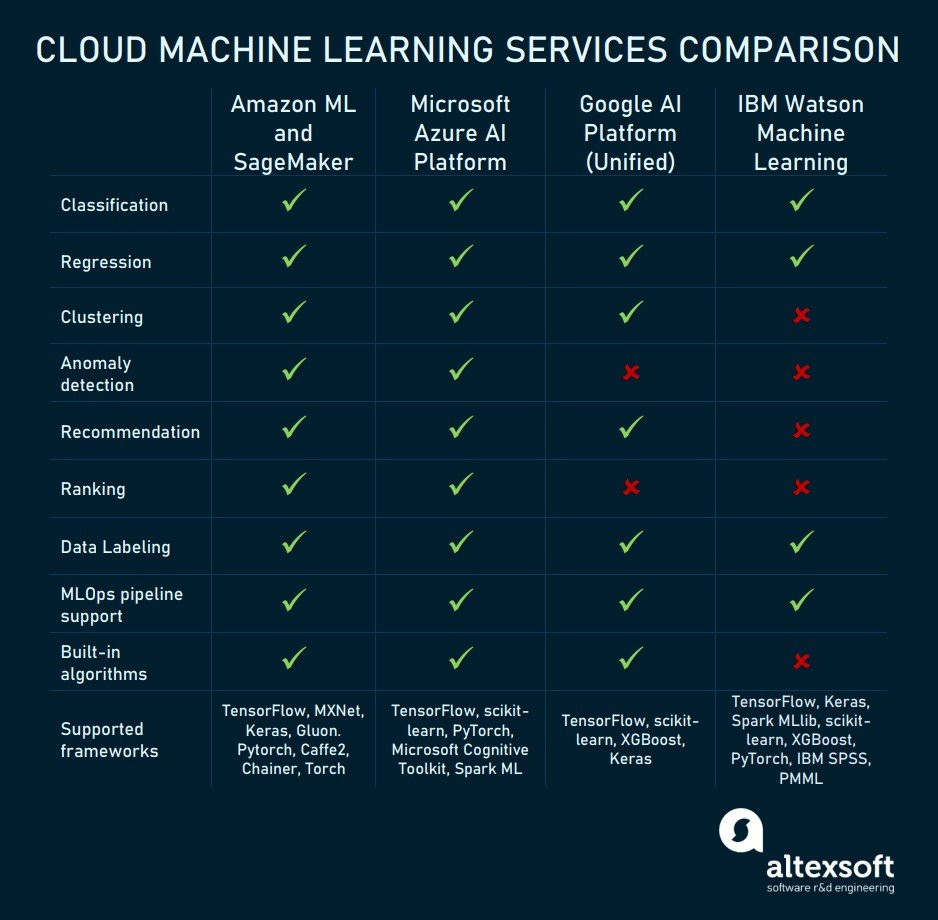
\includegraphics[width=150mm]{./appendices/mlaas-comparison}
    \caption{Machine learning as a Service comparison.~\cite{altexsoft2021mlaas}
    \label{fig:mlaas-comparison}}
\end{figure}

Amazon's new SageMaker service
has replaced the old Amazon Machine Learning service.
It is very much like Azure Machine Learning service
produced by Microsoft.
Azure, however,
has one major advantage
which is the ML Studio environment.
Most of the MLaaS provider's solutions
have some sort of no-code to low-code design features
which makes pipeline designing easy.
Azure ML Studio lets the developer design and deploy
full ML pipelines with drag-and-drop user interface.
Compared to SageMaker and Azure,
Google AI Platform is missing anomaly detection and ranking abilities.
IBM Watson has even less features,
as demonstrated in the table \ref{fig:mlaas-comparison}.\cite{altexsoft2021mlaas}

%% ************************************************************************************************************

\subsection{Azure ML Studio}\label{subsec:bg-azure-ml-studio-algorithms}

Microsoft Azure offers a Machine Learning Studio environment
for easy ML pipeline designing.
ML Studio gives ML designer a possibility to
train algorithms and publish cloud endpoints
utilizing all Azure resources
connecting the power of ML
to all other Azure features
like data storages, IoT-services, and cloud computing.\cite{altexsoft2021mlaas,microsoft2022azureml}

\begin{figure}[htb]
    \centering
    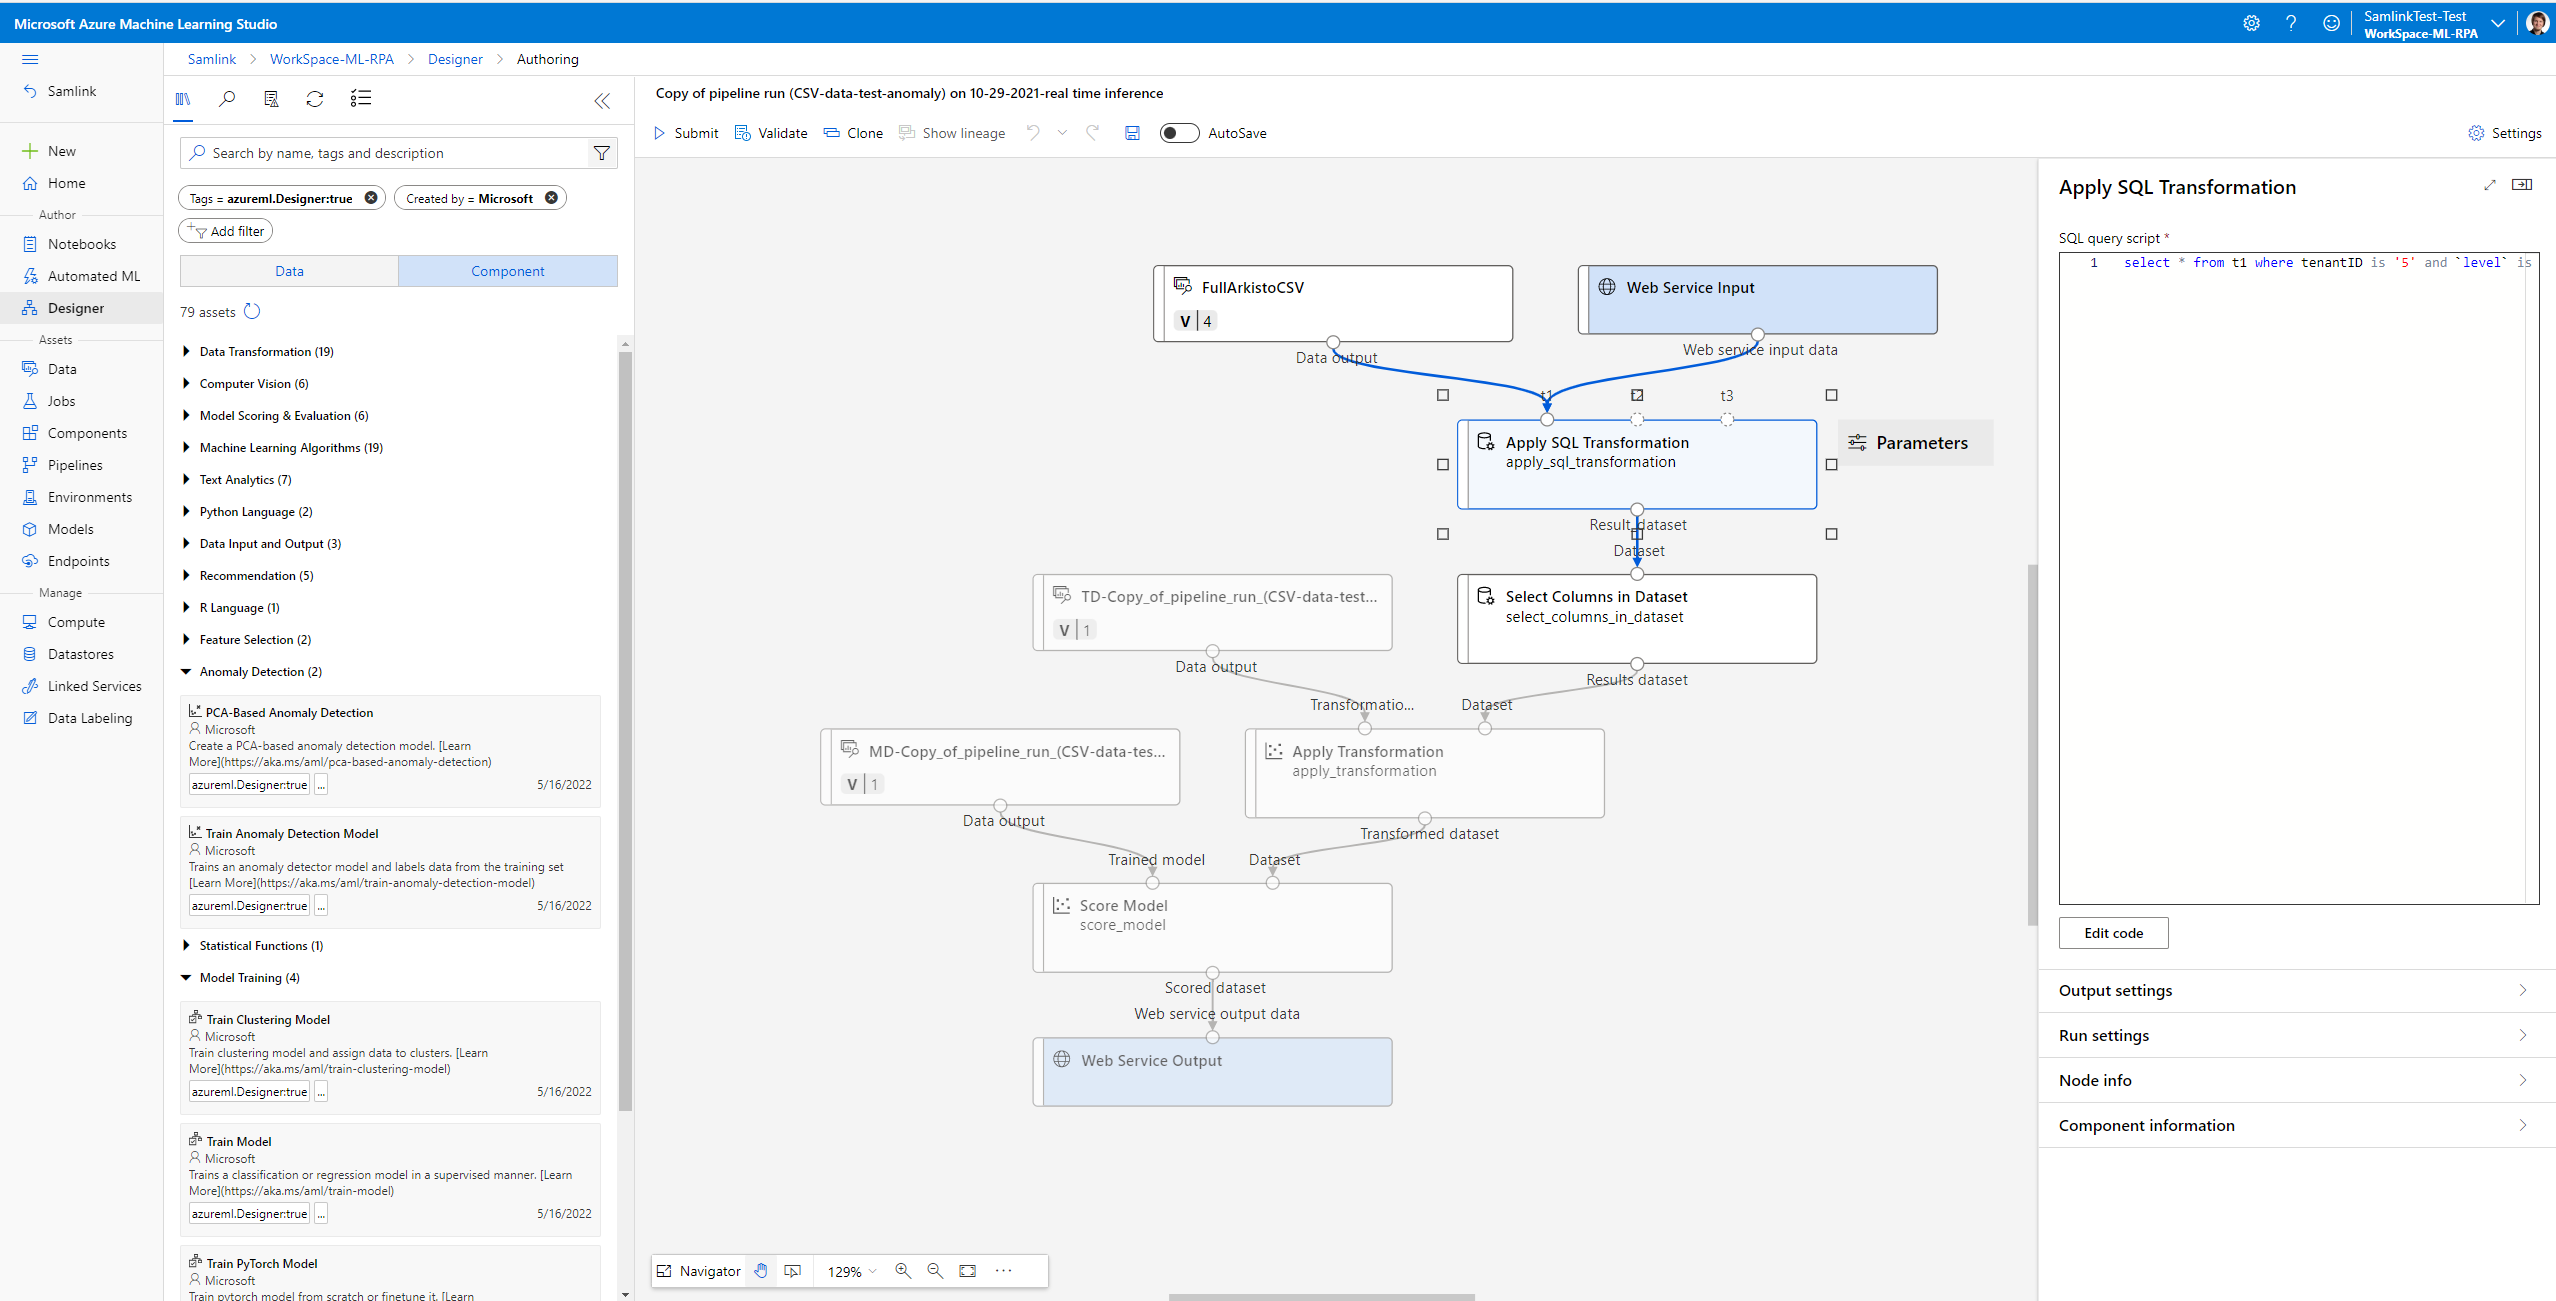
\includegraphics[width=150mm]{./appendices/azure-ml-studio-example}
    \caption{With drag-and-drop pipeline designer
    it is easy to get started with ML programming in Azure ML Studio,
        and visualizing the process helps understand all pipeline components
        and their relations to each other.
    \label{fig:azure-ml-studio-example}}
\end{figure}

Each component in pipeline can be tuned
to a certain extent.
ML Studio has a predefined set of ready algorithms to use.
Example of Azure ML Studio interface
is shown in figure \ref{fig:azure-ml-studio-example}.
Data to the ML Studio environment
can be imported from local storage,
but also from various other Azure services
such as storage accounts with table and blob data.
Trained ML pipeline can be inserted into wider operation chain
combining other Azure services to it.
This allows designer to use ML computing capabilities
with existing production environments
utilizing services like IoT, API, or Kubernetes.


%% ************************************************************************************************************

\subsection{Regression algorithm}\label{subsec:bg-regression-ml}
\todo{science and math behind regression algorithm}
Regression analysis is typical approach in statistical science.
It is used to find relationships with a set of variables.
%% TODO!
%% TODO: REFERENCES!
%% TODO: Mathematical background

%% ************************************************************************************************************

\subsection{PCA-based anomaly detection}\label{subsec:bg-pca-ada}
\todo{Explain PCA and mention other ADA algorithms}
%% TODO: rename subsection if more algorithms are introduced?

Principal Component Analysis, or PCA,
is a machine learning technique
used to analyze data and explain the variance inside it.~\cite{azure2022pca}



Other anomaly detection methods exist, but they are not supported by ML Studio
in a ready component level. %% TODO: check wording.
\todo{Something about Anomaly and Novelty detection differences?}
%% TODO: Mathematical background
%% TODO: How PCA works for anomaly detection? How is it used in it?
%% TODO: Differences for other anomaly detection methods? What other methods are there?

%% TODO!
\todo{placeholder picture. replace with mathematical explanation}
\begin{figure}[htb]
    \centering
    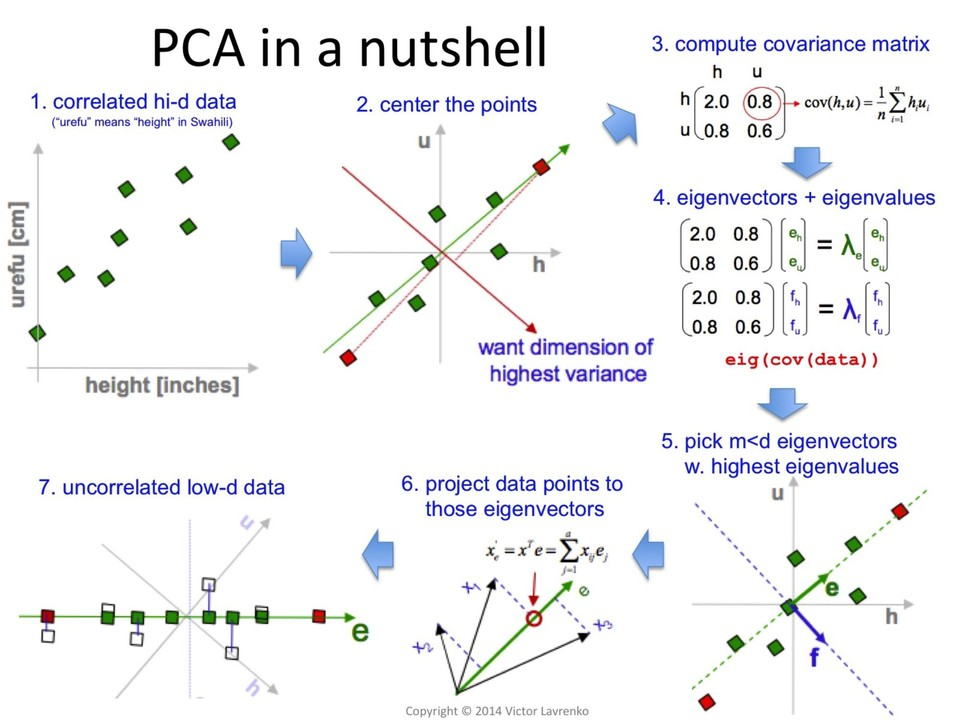
\includegraphics[width=150mm]{./appendices/pca-nutshell}
    \caption{PCA in a nutshell
        \label{fig:pca-nutshell}}
\end{figure}

%% ............................................................................................................

\subsubsection*{One-Class support vector machine}
%% TODO: This is also usable in azure, but not suitable in our case
%% TODO: make sure this is mentioned in places where "only one is pca" is considered

Azure ML Studio has also another anomaly detection algorithm to use.
This module is called One-Class Support Vector Machine.
In our case, however,
this module was not deemed suitable
as the documentation mentioned that
\enquote{The dataset that you use for training
can contain all or mostly normal cases.}
Because the content of the data used did not meet this requirement,
the usage of this component was decided to skip.

%% TODO: https://docs.microsoft.com/en-us/previous-versions/azure/machine-learning/studio-module-reference/one-class-support-vector-machine
%% TODO: add some reference to module

%% ************************************************************************************************************

\subsection{N-gram features and feature hashing}\label{subsec:bg-ngram-features}
%% TODO:
\todo{cover basic n-gram features and ML connection}

\toimhuom{unorganized text below:}
As stated before, %% TODO: state before!
features are the key elements in ML algorithm training.
As textual input does not have any meaning to machines as itself,
it is necessary to create a connection between words and features for algorithm.
In ML training, one typical approach is to convert textual input to numerical features.
For example, by creating a dictionary of words used in the input
and assigning each word an identification number,
we can express words as a count of certain words used.
In addition,
as words include meanings not only individually but also
with relation to each other and in their order, %% TODO: Some example!
we can add more information for the algorithm
by creating word pairs and groups in the dictionary.
These groups are referred as word grams,
where \textbf{n} in n-gram refers to the maximum number of words
in a group of consecutive words in the input sentence.

%% TODO: check above
%% TODO: REFERENCES!
%% TODO: More?
%% TODO: mathematical theories?

\todo{explain feature hashing component functionality briefly}
%% TODO: Clarifying example!

As the number of word grams in a dictionary can increase significantly
in complex input cases,
it is necessary to limit the resource usage by decreasing the features analyzed.
One way to do this is use feature hashing.
This means that instead of pure n-gram count
we use hashed value of several n-grams
thus reducing the amount of features.
As a drawback,
the amount of information might also get reduced as the data is "compressed"
but this way we can include more features for algorithm training
without significant resource demands.

%% TODO: check above
%% TODO: REFERENCES!
%% TODO: More?

%% ************************************************************************************************************

\subsection{Robotic process automation in Samlink}\label{subsec:bg-rpa-in-samlink}
\todo{Short explanation of RPA in Samlink, mostly to clear out the terms used in this study}

Robotic process automation, or RPA,
is used to automate mechanical tasks.
Usually it operates on the UI level
and can be used to repeat meaningful functions
instead of mechanical actions.
For example, with screen recording macros
only position at the screen and mechanical key pressing is recorded and repeated.
RPA automation, however,
is able to repeat the functionalities those actions trigger,
such as inputting text to a certain named field on the UI,
or logging in with given username and password
regardless of the location of those fields on the layout.

\todo{references!}

In Samlink RPA operations,
a central coordinating system called \enquote{Orchestrator}
supervises the RPA processes.

\todo{Add reference to hierarchy picture}

\todo{Dummy picture, replace with better}
\begin{figure}[htb]
    \centering
    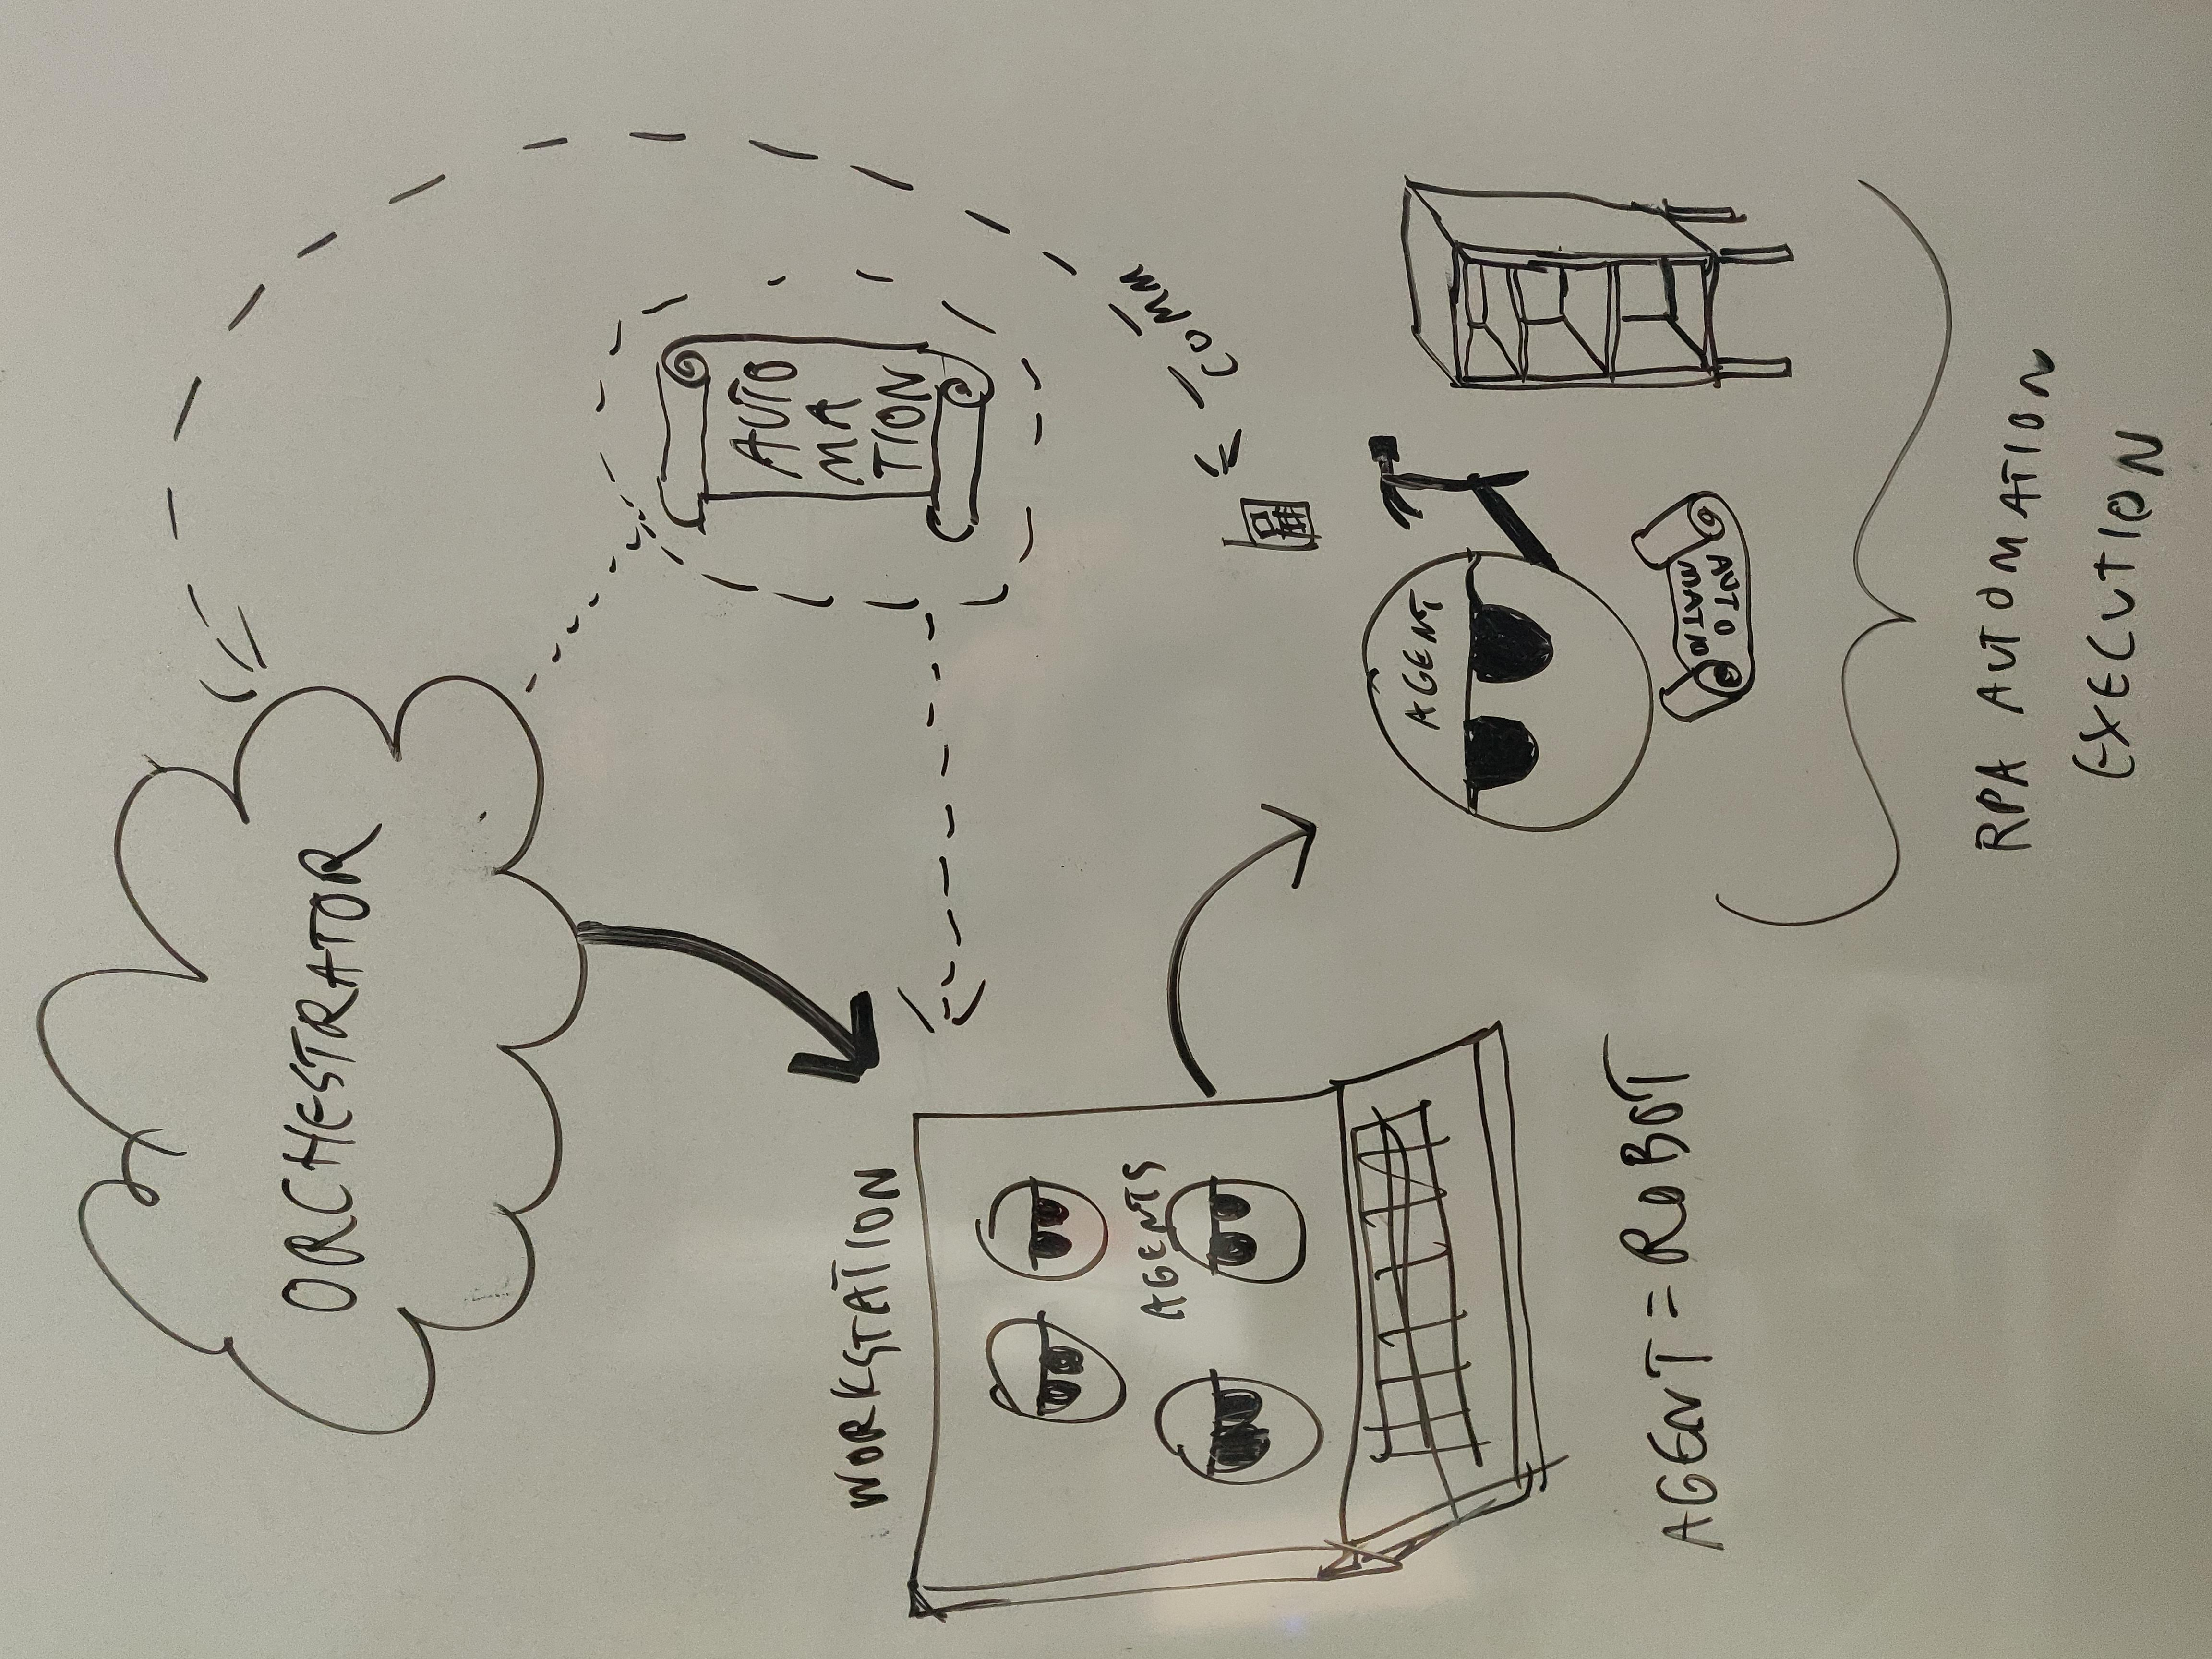
\includegraphics[width=100mm,angle=270]{./appendices/rpa-hierarchy}
    \caption{TODO:! Dummy. To be replaced with proper picture.
    Hierarchy of RPA components explaining the terms and their relations
        \label{fig:rpa-hierarchy}}
\end{figure}



%% ************************************************************************************************************

\subsection{Data sensitivity}\label{subsec:bg-data-sensitivity}
\todo{some basic stuff about anonymization, data sensitivity and data protection}
\todo{Just practicalities, not much about theory or background}

During this study,
it was necessary to make sure no sensitive data
was moved out of the production environment.
This was mostly due to regulations described in GDPR. %% TODO: wording? More?

Data anonymization was executed in production environment
with PowerShell script.
Several predefined identification features were searched with
regular expression (or regex), patterns and replaced with
default keys.
%% TODO: examples
%% TODO: Sources!
%% TODO: How does anonymization affect to ML algorithm functionalities/usages?

%% TODO: references?
%% TODO: Refer to k-anonymization and pseudonymization. Explain BRIEFLY
\begin{itcomment} %% Moved from Methods-section
    Here we could explain more about pseudonymization and k-anonymization,
    but is it necessary as they were not used or considered?
    It would bring something more to the study, of course,
    but is it worth the time?
\end{itcomment}


%% ************************************************************************************************************

\subsection{Log data analyzing with ML}\label{subsec:bg-log-data-analyzing-with-ml}
\todo{Some research should exist}
TODO: In this section, we look
what studies and cases of ML log data analyzing exists in the IT field.
Only briefly, nothing too deep.


%% ************************************************************************************************************

%% TODO: Workname. Check.
\subsection{Random delay in log event analyzing}\label{subsec:bg-random-delay}
\todo{Anything about the topic?}

Random delay in input data features
is not unusual aspect in time-series forecasting.
Time-series in ML context
refers to data features that varies over time
and is usually affected by past values.
As an example,
ML algorithm could try to predict future weather
based on measured temperature and air pressure.
Both these features change over time
and also affect to their own future values.

Random delay in such an example
could be due to some other local or global features
like
%% TODO: find proper exampe about time series forecasting and random delay!
%% TODO: REFERENCES

This study, however,
is not time-series
because the majority of the log rows
are not affected by previously logged events.
Random delay in this case
is caused by banking clerks
finding the issue and writing a technical support request.
This delay can span from hours to several days
depending on the weekday and time the issue occurred.

%% TODO: More to background?

As random delay of such
does not seem to be trivial to take into account
with ML algorithms, %% TODO: Any sources?
a simple method to solve this was used
which we call \enquote{time frame compression method}.
More about this approach is discussed in the section~\ref{subsec:pipe-timeframe-compression-and-statistics}

%% ************************************************************************************************************


\subsection{Hybrid machine learning approach in anomaly detection}\label{subsec:bg-hybrid-ml-approach-with-anomaly-detection}

Hybrid machine learning (HML)
refers to an ML technique
where two or more ML methods are combined
to overcome the limitations of
or to boost the estimation capabilities of
a single method alone.\cite{Anifowose2020hml}
In this study,
we combine PCA-based anomaly detection algorithm
with regression algorithm
in order to amplify the prediction powers of our ML algorithm
when trying to determine the possible ticket count
based on log events.

Hybrid machine learning is not rare technique in ML field.\cite{shon2007hybrid,tsai2010credit,mohan2019effective,
    hsieh2005hybrid,jain2007hybrid,kim2007hybrid,lee2002credit,malhotra2002differentiating}
%% TODO:
\todo{Something about the HML in ADA}

In order to clarify whether hybrid approach is suitable for the current study problem
we will compare the results of hybrid ML technique
with a single ML algorithm usage.


\todo{Include wireframe model about hybrid model}
%% TODO: Include wireframe model about hybrid model


%% TODO: Move to methods section?
With ML algorithm utilizing n-gram features combined with time frame compression
it is possible to get estimates
about the support tickets based on the log events.
It is not feasible to use anomaly detection on its own to do this
as plain sum of anomalies detected
is not correlating with tickets received.

We can, however,
amplify our ticket estimating algorithm with anomaly value features.
As we first count the anomaly numbers with anomaly detection algorithm %% TODO: better wording?
and their calculated statistical features with another algorithm,
like regression algorithm,
we get more relative information to use
when creating the final ticket number estimations. %% TODO: check sensability



\begin{itcomment}
    Hybrid ML as a term is used here to explain that we
    use two different ML algorithms in two separate phases.
    In first phase we try to give an anomaly certainty value for each log row
    using PCA-based anomaly detection component.
    In second phase we use this value as a feature to estimate ticket amount in time range
    by utilizing regression algorithm.

    Dual algorithm approach should not be unusual in ML field,
    but how existing studies or case examples relate to our way is uncertain.

    If nothing exists about the topic (at least nothing easily to be found)
    it should be worth to mention.
    But if there is a lot of case examples about this, it feels unnecessary
    to discus about it in more detail.
\end{itcomment}


\clearpage